\newcommand\scalemath[2]{\scalebox{#1}{\mbox{\ensuremath{\displaystyle #2}}}}

\documentclass{article}
\usepackage{tkz-berge}
\usepackage{amsmath}

\title{Numerical simulation of a bubble cluster}
\author{Tommaso Sciortino}
\date{October 2011}

\begin{document}
\maketitle
\begin{abstract}
We present a scheme for simulating the motion of a collection of 2-dimensional
bubbles which touch at 1-dimensional walls.  In section 1, we introduce a model
where bubble walls are represented as Bezier curves.  Using the
Euler-Lagrange technique, we derive equations of motion for the
control points of the Bezier curves in section 2. Finally, in section 3, we
discuss how those equations can be solved numerically to produce an animation.
\end{abstract}
\clearpage

\section{Representation}
We represent a bubble cluster as a planar graph which partitions the plane
into faces. Each face represents the interior of a bubble. Each edge represents
a wall where two bubbles touch. Vertices occur in the graph where
multiple bubble walls meet at a point.

\begin{figure}[h]
\centering
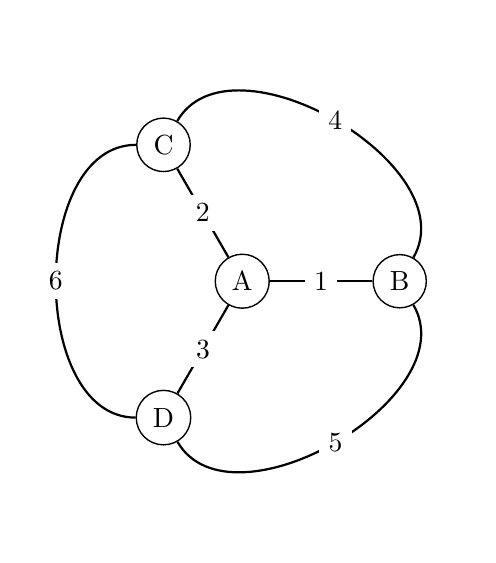
\begin{tikzpicture}[]
\GraphInit[vstyle=Normal] 
\Vertex[]{A}  
\Vertex[a=0, d=2cm]{B} 
\Vertex[a=120, d=2cm]{C}
\Vertex[a=240, d=2cm]{D} 
\Edge[label={1}](A)(B)
\Edge[label={2}](A)(C)
\Edge[label={3}](A)(D)
\Edge[style={bend left=90}, label={4}](C)(B)
\Edge[style={bend left=90}, label={5}](B)(D)
\Edge[style={bend left=90}, label={6}](D)(C) 
\end{tikzpicture}
\caption{A planar cubic graph}
\end{figure}

Since more than one wall may connect the same two vertices the graph is a
multigraph. Furthermore, since only vertices where three walls meet 
are physically stable we will constrain the graph to be 3-regular or ``cubic''.
Similarly, loops are physically unstable and thus disallowed.

\subsection{Bubbles as faces}
Each bubble face can be defined by the ring of serially connected edges which
form its border. Consequently each edge belongs to two faces. In addition to
the normal internal faces there is one external face which represents the air
outside the bubble cluster.

\begin{figure}[h]
\centering
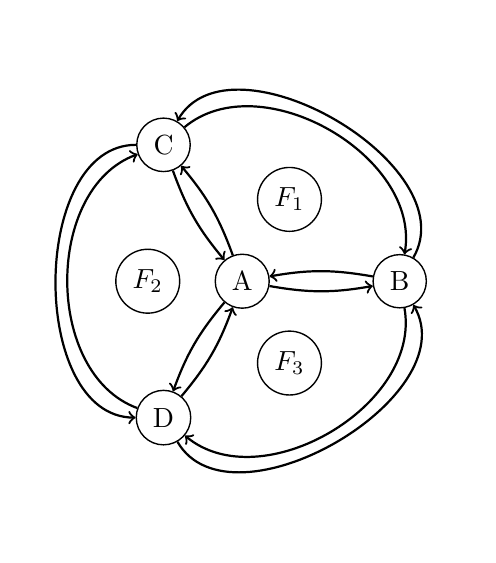
\begin{tikzpicture}[]
\GraphInit[vstyle=Normal] 
\Vertex[]{A}  
\Vertex[a=0, d=2cm]{B} 
\Vertex[a=120, d=2cm]{C}
\Vertex[a=240, d=2cm]{D} 
\Vertex[Math, a=60, d=1.2cm]{F_1}
\Vertex[Math, a=180, d=1.2cm]{F_2}
\Vertex[Math, a=300, d=1.2cm]{F_3} 
\Edge[style={<-,bend left=10}](A)(B)
\Edge[style={->,bend right=10}](A)(B)
\Edge[style={<-,bend left=10}](A)(C)
\Edge[style={->,bend right=10}](A)(C)
\Edge[style={<-,bend left=10}](A)(D)
\Edge[style={->,bend right=10}](A)(D)
\Edge[style={<-,bend left=90}](C)(B)
\Edge[style={->,bend left=70}](C)(B)
\Edge[style={<-,bend left=90}](B)(D)
\Edge[style={->,bend left=70}](B)(D)
\Edge[style={<-,bend left=90}](D)(C)
\Edge[style={->,bend left=70}](D)(C) 
\end{tikzpicture}
\caption{A directed graph representation}
\end{figure}

If we view each edge as a pair of directed edges - one in each direction - then
each face can be defined as a list of directed edges where the head of each
is the tail of the next. Consequently, each directed edge belongs to exactly
one face and (except for the external face) the directed edges of each face all
run clockwise. This convention is useful for properly calculating various quantities
when we need to integrate around a face in the right order and direction.
\subsection{Bubble walls as cubic Bezier curves}
The position of a bubble wall is represented by a cubic Bezier curve defined as
a parametric equation with four control points $\vec{B_n}(t)$
\begin{align}
\vec{B}(p,t)=(1-p)^3\vec{B_0}(t)+3p(1-p)^2\vec{B_1}(t)+3p^2(1-p)\vec{B_2}(t)+p^3\vec{B_3}(t)
\end{align}
The parameter p runs from 0 to 1. We also define
\begin{align}
\vec{B}(p,t)&=B_x(p,t)\hat{x} +B_y(p,t)\hat{y}
\end{align}
and
\begin{subequations}
\begin{align}
B_x(p,t)&=(1-p)^3x_0(t)+3p(1-p)^2x_1(t)+3p^2(1-p)x_2(t)+p^3x_3(t)\\
B_y(p,t)&=(1-p)^3y_0(t)+3p(1-p)^2y_1(t)+3p^2(1-p)y_2(t)+p^3y_3(t)
\end{align}
\end{subequations}
In terms of the directed edge representation, one directed edge traverses the
curve as p goes from 0 to 1, the other from 1 to 0.
\clearpage
\section{Physics}
The position of a bubble cluster's walls at any time $t$ is given by the
positions of the control points. We denote these as
$q_1(t),q_2(t),\dots,q_n(t)$. To find how the walls change with time we must
numerically solve for these functions.

To derive equations of motion we use Lagrangian mechanics. We define the
Lagrangian $\mathcal{L}_T=K_T-V_T$ as the total kinetic minus total potential
energy of the system. The equations of motion are the path for which the
integral of the Lagrangian over time is stationary. To find these we generate
the following equations:
\begin{align}
\frac{d}{d t}\frac{\partial \mathcal{L}_T}{\partial q'_i}
=\frac{\partial
\mathcal{L}_T}{\partial q_i} \qquad \text{for each } q_i
\end{align} 

Taken together these yield a nonlinear system of ordinary differential
equations.
\subsection{Kinetic Energy}
To find the kinetic energy we first determine the velocity of every point on a
bubble wall. To do this we take the derivative of the position with respect to
time.
\begin{displaymath}
\vec{B}'(p,t)=(1-p)^3\vec{B_0}'(t)+3p(1-p)^2\vec{B_1}'(t)+3p^2(1-p)\vec{B_2}'(t)+p^3\vec{B_3}'(t)
\end{displaymath}
To have kinetic energy the wall must have mass so we introduce a coefficient
$m$ to represent mass per unit interval of the parameter p. This gives us the kinetic energy at the
infinitesimal point p
\begin{displaymath}
K(p,t) = \frac{m}{2} \left|\vec{B}'(p,t)\right|^2
\end{displaymath}
To find the total kinetic energy for the bubble wall we integrate over the
length of the wall
\begin{align*}
K(t)&= \int_0^1 \frac{m}{2} \left|\vec{B}'(p,t)\right|^2 dp\\
&=\frac{m}{2} \int_0^1 \left(\sqrt{B'_x(p,t)^2+B'_y(p,t)^2}\right)^2 dp\\
&=\frac{m}{2} \int_0^1 B'_x(p,t)^2+B'_y(p,t)^2 dp
\end{align*}
In terms of the derivatives of the coordinates of the 4 control points $x_n(t)$
and $y_n(t)$ we get:
\begin{align*}
K(t)=\frac{m}{2} \int_0^1
\left((1-p)^3x'_0+3p(1-p)^2x'_1+3p^2(1-p)x_2'+p^3x'_3\right)^2 \\
 \quad+ \left((1-p)^3y'_0+3p(1-p)^2y'_1+3p^2(1-p)y'_2+p^3y'_3
\right)^2 dp
\end{align*}
Integrating gives us
\begin{align*}
K(t)=\frac{m}{2} &\left( 
\frac{x_0^{'2}}{7} + \frac{x'_0 x'_1}{7} + \frac{2 x'_0 x'_2}{35} + 
\frac{x'_0 x'_3}{70}  + \frac{3 x_1^{'2}}{35} \right.\\
&\left.\quad +\frac{9 x'_1 x'_2}{70} 
+ \frac{2 x'_1 x'_3}{35} + \frac{3 x_2^{'2}}{35} + \frac{x'_2 x'_3}{7} +\frac{x_3^{'2}}{7}\right.\\
&\quad\left. +\frac{y_0^{'2}}{7} + \frac{y'_0 y'_1}{7} + \frac{2 y'_0 y'_2}{35} + 
\frac{y'_0 y'_3}{70} + \frac{3 y_1^{'2}}{35} \right.\\
&\left.\quad  +\frac{9 y'_1 y'_2}{70} 
+ \frac{2 y'_1 y'_3}{35} + \frac{3 y_2^{'2}}{35} + \frac{y'_2 y'_3}{7}
+\frac{y_3^{'2}}{7}\right)
\end{align*}
Rephrased more clearly with matrices
\begin{align}
K(t)=
\frac{m}{140} &\left(
\begin{bmatrix} x'_0 & x'_1 & x'_2 & x'_3 \end{bmatrix}
 \begin{bmatrix} 
10 & 10 & 4 & 1\\
0 & 6 & 9 & 4\\
0 & 0 & 6 & 10\\
0 & 0 & 0 & 10\\ 
\end{bmatrix}
\begin{bmatrix} x'_0\\x'_1\\x'_2\\x'_3 \end{bmatrix}
\right.\\
&+ \left.
\begin{bmatrix} y'_0 & y'_1 & y'_2 & y'_3 \end{bmatrix}
 \begin{bmatrix} 
10 & 10 & 4 & 1\\
0 & 6 & 9 & 4\\
0 & 0 & 6 & 10\\
0 & 0 & 0 & 10\\ 
\end{bmatrix}
\begin{bmatrix} y'_0\\y'_1\\y'_2\\y'_3 \end{bmatrix} 
\right)\nonumber
\end{align}
Note that $K$ is just for one bubble wall. To get the total
kinetic energy of the system $K_T$ we must sum the kinetic energy of all the
walls. Note too that each Bezier curve end point is shared by the other walls
meeting at that vertex. This means that some coordinates $q_i$ will appear in
more than one wall's kinetic energy equation.
\subsection{Potential Energy}
Potential energy in our system comes from two sources, air pressure and surface
tension. Surface tension potential rises as a wall lengthens.
Air pressure potential rises as the air inside a bubble is compressed.
\subsubsection{Air Pressure Potential}
We use the ideal gas law to estimate the
behavior of the gas in the bubble under pressure. Here $P(t)$ and $A(t)$ are
pressure and area of the bubble, $T$ the temperature, $N$ the number of particles in the
gas, and $k$ is Boltzmann's constant (modified for 2 dimensions). We will assume
that all processes are isothermal and that $N$ is constant.
\begin{align*}
P(t)=\frac{NkT}{A(t)}=\frac{constant}{A(t)}
\end{align*}
The energy necessary to change a bubble's area from $A_1$ to $A_2$ is
\begin{align*}
\Delta E = \int_{A_1}^{A_2} P dA = \int_{A_1}^{A_2} \frac{NkT}{A} dA = NkT
\ln\left(\frac{A_2}{A_1}\right)
\end{align*}
We define the ambient pressure of the outside air as $\rho$, and $A_\rho$ as
the area of the bubble at this pressure. Then the energy stored as
potential in a bubble of area $A(t)$ is
\begin{align}
V_p(t) = -\rho A_\rho \ln\left(\frac{A(t)}{A_\rho}\right) = \rho A_\rho
\ln\left(\frac{A_\rho}{A(t)}\right)
\end{align}

Though the above formula works for normal bubbles, we must deal separately with
the air outside the bubble cluster represented by the external face. Since
the area of this bubble is infinite, the formula will not apply directly.
However, if we first set the bubble cluster in a large (but finite) room and
then take the limit as the room becomes infinitely large, we can get a
well-defined formula for the energy. 

Let $A_r$ be the area of the room and $A_m$ be the area of the bubble mass. Then
the area of the external bubble is $A_r-A_m$ and the energy required to go from
$A_r$ to $A_r-A_m$ is
\begin{align}
V_p(t) = \lim_{A_r\to\infty} \rho A_r \ln\left(\frac{A_r}{A_r-A_m(t)}\right)=
\rho A_m(t)
\end{align}

All that remains is to determine the area of the bubble. This is simply the sum
of the signed area under the curves that make it up. The formula for the area
under a Bezier curve is
\begin{align*}
A_b &= \int_0^1 B_y(p)\frac{\partial B_x(p)}{dp} dp\\
&=\int_0^1
\left((1-p)^3y_0+3p(1-p)^2y_1+3p^2(1-p)y_2+p^3y_3\right)\\
&\quad \left(-3(1-p)^2x_0 +3(1+p(3p-4))x_1+3p(2-3p)x_2 +3p^2x_3\right)dp\\
&= x_0\left( \frac{-y_0}{2}+ \frac{-3y_1}{10}+\frac{-3y_2}{20}+\frac{-y_3}{20}\right)\\
&+ x_1\left(\frac{3y_0}{10}+ \frac{-3y_2}{20} +\frac{-3y_3}{20}\right)\\
&+ x_2\left(\frac{3y_0}{20}+ \frac{3y_1}{20} +\frac{-3y_3}{10}\right)\\
&+ x_3\left(\frac{y_0}{20} + \frac{3y_1}{20} +\frac{3y_2}{10}
+\frac{y_3}{2}\right)
\end{align*}
Rephrased more succinctly with matrices:
\begin{align}
A_b=
\frac{1}{20} 
\begin{bmatrix} x_0 & x_1 & x_2 & x_3 \end{bmatrix}
\begin{bmatrix} 
-10 & -6 & -3 & -1\\
6 & 0 & -3 & -3\\
3 & 3 & 0 & -6\\
1 & 3 & 6 & 10\\ 
\end{bmatrix}
\left[ \begin{array}{c} y_0\\y_1\\y_2\\y_3 \end{array} \right] 
\end{align}

To determine the area of a bubble from the area under the curves that make it up
one must be careful to integrate each wall in the right direction. Here, the
directed edge view is very useful in avoiding sign errors.

Of course to get the total potential due to pressure we need to sum over all
walls of all bubbles in the cluster.
\subsubsection{Surface Tension Potential}
The potential energy due to surface tension varies linearly with wall length. We
will introduce a coefficient $\tau$ for energy per unit length.
\begin{align}
V_s(t)&=\tau Length(B)\\
&=\tau \int_0^1 \left|\frac{d \vec{B}(p,t)}{dp}\right| dp \nonumber\\
&=\tau \int_0^1 \sqrt{\left(\frac{d B_x(p,t)}{dp}\right)^2+\left(\frac{d
B_y(p,t)}{dp}\right)^2} dp \nonumber
\end{align}
where
\begin{align*}
\frac{d B_x(p,t)}{dp}&= -3(1-p)^2x_0 +3(3p-1) (p-1)x_1+3p(2-3p)x_2 +3p^2x_3\\
\frac{d B_y(p,t)}{dp}&= -3(1-p)^2y_0 +3(3p-1) (p-1)y_1+3p(2-3p)y_2 +3p^2y_3
\end{align*}
The integral is of the square root of a 4th degree polynomial in p. This is
known as an ``elliptic integral'' and cannot generally be solved in closed
form.
\subsection{Calculating the equations of motion}
Having calculated the kinetic and potential energy of the system we can finally
use them to calculate the Lagrangian $\mathcal{L}_T=K_T-V_T$.

Observe that the formula for kinetic energy is defined only in terms of
the velocities of the control points $q'_1,\dots,q'_n$ and the potential is
defined only in terms of positions of the control points $q_1,\dots,q_n$.
This simplifies the equations of motion greatly:
\begin{align*}
\frac{d}{d t}\frac{\partial \mathcal{L}_T}{\partial q'_n} 
&=\frac{\partial \mathcal{L}_T}{\partial q_n} \\
\frac{d}{d t}\frac{\partial (K_T-V_T)}{\partial q'_n}
&= \frac{\partial (K_T-V_T)}{\partial q_n} \\
\frac{d}{d t}\left( \frac{\partial K_T}{\partial q'_n} - \frac{\partial
V_T}{\partial q'_n}\right)
&=\frac{\partial K_T}{\partial q_n}-\frac{\partial V_T}{\partial q_n} \\
\frac{d}{d t} \frac{\partial K_T}{\partial q'_n}
&=-\frac{\partial V_T}{\partial q_n}\\
\frac{d}{d t} \frac{\partial K_T}{\partial q'_n}
&= -\left(\frac{\partial V_{Tp}}{\partial q_n}+\frac{\partial V_{Ts}}{\partial
q_n}\right)
\end{align*}
To get the equations of motion we need to calculate the above equation for every
control point coordinate in the system. This means generating 8 equations for
every bubble wall in the system. We will only work out 2 such equations here as
the rest can be inferred from them by symmetry.
\subsubsection{Equation of motion for $x_1$}
We will generate the Lagrangian for the x coordinate of the second control
point $x_1$ of the bubble wall as this case is simpler than the first
coordinate which is shared by three walls.  Our equation is
\begin{align*}
 \frac{d}{d t} \frac{\partial K_T}{\partial x'_1} =-\left(\frac{\partial
 V_{Ts}}{\partial x_1} + \frac{\partial V_{Tp}}{\partial x_1}\right)
\end{align*}

First observe that since $x_1$ only appears in the kinetic energy formula for
one wall the quantity $\frac{\partial K_T}{\partial x'_1}=\frac{\partial K}{\partial x'_1}$
 so the left-hand side of the equation is 
\begin{align*}
\frac{d}{d t} \frac{\partial K_T}{\partial x'_1} &=
\frac{d}{d t} \frac{\partial K}{\partial x'_1}\\
 &= \frac{d}{d t}
 \frac{\partial }{\partial x'_1} \frac{m}{140} \left(
\begin{bmatrix} x'_0 & x'_1 & x'_2 & x'_3 \end{bmatrix}
 \begin{bmatrix} 
10 & 10 & 4 & 1\\
0 & 6 & 9 & 4\\
0 & 0 & 6 & 10\\
0 & 0 & 0 & 10\\ 
\end{bmatrix}
\begin{bmatrix} x'_0\\x'_1\\x'_2\\x'_3 \end{bmatrix}
\right.\\
&\qquad\qquad\qquad+ \left.
\begin{bmatrix} y'_0 & y'_1 & y'_2 & y'_3 \end{bmatrix}
 \begin{bmatrix} 
10 & 10 & 4 & 1\\
0 & 6 & 9 & 4\\
0 & 0 & 6 & 10\\
0 & 0 & 0 & 10\\ 
\end{bmatrix}
\begin{bmatrix} y'_0\\y'_1\\y'_2\\y'_3 \end{bmatrix} 
\right)\\ 
&= \frac{m}{140} \frac{d}{d t}\left(10x'_0+12x'_1+9x'_2+4x'_3 \right)\\
&= \frac{m}{140} \left(10x''_0+12x''_1+9x''_2+4x''_3 \right)
\end{align*}

The right-hand side has two parts. One for pressure and one for surface tension. We
calculate the pressure first. 

Observe that $x_1$ only appears in the formula for the areas of the bubbles
$A_1$ and $A_2$ on either side of the bubble wall. Let $A_{1\rho}$ and
$A_{2\rho}$ be their area at ambient pressure. 
\begin{align*}
\frac{\partial V_{Tp}}{\partial x_1} &= \frac{\partial }{\partial x_1}
\left(
\rho A_{1\rho}
\ln\left(\frac{A_{1\rho}}{A_1}\right)
+\rho A_{2\rho}
\ln\left(\frac{A_{2\rho}}{A_2}\right)
\right)\\
&= 
\rho \left(
\frac{A_{1\rho}}{A_1} \frac{\partial A_1}{\partial x_1}
+\frac{A_{2\rho}}{A_2} \frac{\partial A_2}{\partial x_1}
\right)
\end{align*}
Note that for one bubble the wall corresponds to a directed edge where p runs
from 0 to 1, for the other it runs 1 to 0. This introduces a sign change in the
formula for area. Let us arbitrarily choose $A_2$ to represent the reversed sign
bubble.
\begin{align*}
\frac{\partial V_{Tp}}{\partial x_1} &= 
\rho \left(
\frac{A_{1\rho}}{A_1} \frac{3}{20}(2y_0-y_2-y_3)
-\frac{A_{2\rho}}{A_2} \frac{3}{20}(2y_0-y_2-y_3)
\right)\\
&= 
 \frac{3\rho}{20} (2y_0-y_2-y_3)
\left( \frac{A_{1\rho}}{A_1} -\frac{A_{2\rho}}{A_2}\right)
\end{align*}
Lastly, observe that for the external face the factor $\frac{A_{\rho}}{A}$ is
instead 1.

Finally we get to the surface tension. Unfortunately this expression is
irreducible.
\begin{align*}
\frac{\partial V_s(t)}{\partial x_1}&=
\frac{\partial}{\partial x_1}
\tau \int_0^1 \sqrt{\left(\frac{d B_x(p,t)}{dp}\right)^2+\left(\frac{d
B_y(p,t)}{dp}\right)^2} dp\\
&=
\tau\int_0^1\frac{\left(\frac{\partial}{\partial x_1}\frac{d
B_x(p,t)}{dp}\right) \frac{d B_x(p,t)}{dp}}{
  \sqrt{\left(\frac{d B_x(p,t)}{dp}\right)^2+\left(\frac{d
B_y(p,t)}{dp}\right)^2}} dp\\
&=
\tau\int_0^1\frac{3(3p-1)(p-1)  \frac{d B_x(p,t)}{dp}}{
  \sqrt{\left(\frac{d B_x(p,t)}{dp}\right)^2+\left(\frac{d
B_y(p,t)}{dp}\right)^2}} dp
\end{align*}
This value must be estimated by numerical integration.

Altogether, that gives us
\begin{align}
\frac{m}{140} \left(10x''_0+12x''_1+9x''_2+4x''_3 \right) &= 
 \frac{3\rho}{20} (2y_0-y_2-y_3)
\left( \frac{A_{1\rho}}{A_1} -\frac{A_{2\rho}}{A_2}\right)\\
&+\tau\int_0^1\frac{3(3p-1)(p-1)  \frac{d B_x(p,t)}{dp}}{
  \sqrt{\left(\frac{d B_x(p,t)}{dp}\right)^2+\left(\frac{d
B_y(p,t)}{dp}\right)^2}} dp \nonumber
\end{align}
\subsection{Equation of motion for $x_0$}
We generate the equation of motion for the x coordinate of a vertex $x_0$ where
three walls meet. We will use $\alpha$, $\beta$, and $\gamma$ to distinguish the
three walls.

The left-hand side of the Lagrangian equation is 
\begin{align}
\frac{d}{d t} \frac{\partial K_T}{\partial x'_0}&=
\frac{m}{140}  \left( 20x''_0+10x''_{1\alpha}+4x''_{2\alpha}+x''_{3\alpha} \right)\\
&\qquad\qquad +\frac{m}{140}\left(
20x''_0+10x''_{1\beta}+4x''_{2\beta}+x''_{3\beta}\right)\nonumber\\ 
&\qquad\qquad +\frac{m}{140} \left(
20x''_0+10x''_{1\gamma}+4x''_{2\gamma}+x''_{3\gamma} \right)\nonumber\\
 &=\frac{m}{140} \left(
60x''_0
+10(x''_{1\alpha}+x''_{1\beta}+x''_{1\gamma})\right.\nonumber\\
&\qquad\qquad \left.+4(x''_{2\alpha}+x''_{2\beta}+x''_{2\gamma})
+(x''_{3\alpha}+x''_{3\beta}+x''_{3\gamma}) \right)\nonumber
\end{align}

For the pressure part of the right-hand side we denote the area of the bubble
shared by $\alpha$ and $\beta$ by $A_{\alpha\beta}$.

\begin{align*}
\frac{\partial V_{Tp}}{\partial x_1} &= 
\rho \left(
\frac{A_{\alpha\beta\rho}}{A_{\alpha\beta}} \frac{\partial
A_{\alpha\beta}}{\partial x_0} 
+\frac{A_{\beta\gamma\rho}}{A_{\beta\gamma}} \frac{\partial
A_{\beta\gamma}}{\partial x_0} 
+\frac{A_{\gamma\alpha\rho}}{A_{\gamma\alpha}} \frac{\partial
A_{\gamma\alpha}}{\partial x_0} 
\right)
\end{align*}
Where
\begin{align*}
\frac{\partial A_{\alpha\beta}}{\partial x_0}=\frac{1}{20}
\left(-10(y_{0\alpha}+y_{0\beta})-6(y_{1\alpha}+y_{1\beta})
-3(y_{2\alpha}+y_{2\beta})-(y_{3\alpha}+y_{3\beta})\right)
\end{align*}

For the tension part of the right-hand side we have
\begin{align*}
\frac{\partial V_s(t)}{\partial x_0}&=
\tau\left(\int_0^1\frac{3(1-p)^2  \frac{d B_{\alpha x}}{dp}}{
  \sqrt{\left(\frac{d B_{\alpha x}}{dp}\right)^2+\left(\frac{d
B_{\alpha y}}{dp}\right)^2}} dp\right.\\
&\qquad \left.+\int_0^1\frac{3(1-p)^2  \frac{d B_{\beta x}}{dp}}{
  \sqrt{\left(\frac{d B_{\beta x}}{dp}\right)^2+\left(\frac{d
B_{\beta y}}{dp}\right)^2}} dp\right.\\
&\qquad \left.+\int_0^1\frac{3(1-p)^2  \frac{d B_{\gamma x}}{dp}}{
  \sqrt{\left(\frac{d B_{\gamma x}}{dp}\right)^2+\left(\frac{d
B_{\gamma y}}{dp}\right)^2}} dp
\right)
\end{align*}

Putting these together to form the equation of motion is left as an exercise to
the reader.
\subsection{Solving the equations of motion}
We are now able to produce the equations of motion; all that is left is to solve
them. The equations can't be written in closed form, so it's unsurprising that
they can't be solved in closed form either. Instead we'll use a slightly
modified form of the forward Euler method for approximating the solution to ODEs.

Observe that for every generalized coordinate $q_j$ we get one equation of the
form:
\begin{align*}
\sum_i^n c_{ij}q_i''(t) = F_j(q_1,q_2,\ldots)
\end{align*}
Here $c_{ij}$ is a coefficient determined in equations (10) and (11) and $F_j$
is $-\frac{\partial V(t)}{\partial q_j}$. We generalize $F_j$ to the vector
function $\vec{F}$ and express the equation in matrix form:
\begin{align*}
C \vec{q''}= \vec{F}(\vec{q})
\end{align*}

Since equations generated for x coordinates only include the second derivative
of x coordinates (and vice versa) this equation can be cut into two, one for x
and one for y.

Now all that is left is to numerically solve. We start with initial positions
and velocities $\vec{q}(t_0)$ and $\vec{q'}(t_0)$. At each step we calculate the
state after time $\Delta t$,  $\vec{q'}(t_{n+1})$ and $\vec{q}(t_{n+1})$ from
$\vec{q}(t_n)$ and $\vec{q'}(t_n)$.
\begin{align*}
\vec{q''}(t_n) &= \vec{F}(\vec{q}(t_n)) / C\\
\vec{q'}(t_{n+1}) &= \vec{q'}(t_n)+\Delta t \vec{q''}(t_n)\\
\vec{q}(t_{n+1}) &= \Delta t \left( \frac{\vec{q'}(t_{n+1}) + \vec{q'}(t_n)}{2}
\right)+ \vec{q}(t_n)
\end{align*}
(Note the matrix division in the first step.)

One final step is to introduce friction. This not only adds realism, but also
helps keep the numerical solution stable. Friction will be modeled by
a drag friction $c_f$ which is proportional to velocity. It modifies the
equations like so:
\begin{align*}
\vec{q'}(t_{n+1}) &= \vec{q'}(t_n)+\Delta t \left(\vec{q''}(t_n)
-c_f\vec{q'}(t_n)\right)\\
&= \left(1-\Delta t c_f\right)\vec{q'}(t_n)+\Delta t \vec{q''}(t_n)
\end{align*}

\subsubsection{Simplifying the matrix equation}

The most time-consuming step in calculating each frame is to solve the matrix equation:

\begin{align*}
C \vec{Q} &= \vec{F}\\
\vec{Q} &=
\begin{bmatrix} 
\vec{Q_c} \\ 
\vec{Q_v}
\end{bmatrix}\\
\vec{F} &=
\begin{bmatrix} 
\vec{F_c} \\ 
\vec{F_v}
\end{bmatrix}
\end{align*}

We begin by looking at the structure of $C$. Here is one example of a 3 bubble cluster:
\begin{align*}
C = \frac{1}{140} \left(
    \scalemath{0.8}{
 \begin{array}{cccccccccccc|cccc}
12& 9& & & & & & & & & & & 4&10& & \\
 9&12& & & & & & & & & & &10& 4& & \\
 & &12& 9& & & & & & & & & 4& & &10\\
 & & 9&12& & & & & & & & &10& & & 4\\
 & & & &12& 9& & & & & & & 4& &10& \\
 & & & & 9&12& & & & & & &10& & 4& \\
 & & & & & &12& 9& & & & & &10& 4& \\
 & & & & & & 9&12& & & & & & 4&10& \\
 & & & & & & & &12& 9& & & & &10& 4\\
 & & & & & & & & 9&12& & & & & 4&10\\
 & & & & & & & & & &12& 9& & 4& &10\\
 & & & & & & & & & & 9&12& &10& & 4\\ \hline
4&10& 4&10& 4&10& & & & & & &60& 1& 1& 1\\
10& 4& & & & &10& 4& & & 4&10& 1&60& 1& 1\\
 & & & &10& 4& 4&10&10& 4& & & 1& 1&60& 1\\
 & &10& 4& & & & & 4&10&10& 4& 1& 1& 1&60\\
\end{array}
}
\right)
\end{align*}

For convenience the zeros have been left empty and the equations of motion have been ordered 
with all the inner control points (in matching pairs) before the vertices. Lines have been 
added to clarify that $C$ is a block matrix of form:

\begin{align*}
C=\left[
\begin{array}{c|c}
A & B \\ \hline
B^{\top} & D
\end{array}\right]
\end{align*}

Our submatrices have very simple forms:
\begin{align*}
A_{ij} &= \left\{ 
  \begin{array}{l l}
    \frac{3}{35} & \quad \text{if $i=j$}\\
    \frac{9}{140} & \quad \text{if control points $i$ and $j$ lie on the same edge}\\
    0 & \quad \text{otherwise}\\
  \end{array} \right.\\
B_{ij} &= \left\{ 
  \begin{array}{l l}
    \frac{1}{14} & \quad \text{if control point $i$ is directly connected to vertex $j$}\\
    \frac{1}{35} & \quad \text{if control point $i$ is indirectly connected to vertex $j$}\\
    0 & \quad \text{otherwise}\\
  \end{array} \right.  \\ 
D_{ij} &= \left\{ 
  \begin{array}{l l}
    \frac{3}{7} & \quad \text{if $i=j$}\\
    \frac{n}{140} & \quad \text{if $i\neq j$}\\
    & \quad \text{where $n$ is the number of edges shared by vertex $i$ and $j$}
  \end{array} \right.
\end{align*}

By block LU decomposition we can show:

\begin{align*}
C=
\begin{bmatrix} 
A & B \\ 
B^{\top} & D
\end{bmatrix} 
=
\begin{bmatrix} 
I & 0 \\ 
B^{\top}A^{-1} & I
\end{bmatrix}   
\begin{bmatrix} 
A & 0 \\ 
0 & D - B^{\top}A^{-1}B
\end{bmatrix}   
\begin{bmatrix} 
I & A^{-1}B \\ 
0 & I
\end{bmatrix}   
\end{align*}
 
To solve $C\vec{Q}=\vec{F}$ let us define 
\begin{align*}
\begin{bmatrix} 
\vec{Q_{2c}} \\ 
\vec{Q_{2v}}
\end{bmatrix}   
=
\begin{bmatrix} 
A & 0 \\ 
0 & D - B^{\top}A^{-1}B
\end{bmatrix}   
\begin{bmatrix} 
I & A^{-1}B \\ 
0 & I
\end{bmatrix}
\begin{bmatrix} 
\vec{Q_c} \\ 
\vec{Q_v}
\end{bmatrix}   
\end{align*}
so we get
\begin{align*}
\begin{bmatrix} 
I & 0 \\ 
B^{\top}A^{-1} & I
\end{bmatrix}   
\begin{bmatrix} 
\vec{Q_{2c}} \\ 
\vec{Q_{2v}}
\end{bmatrix}   
= 
\begin{bmatrix} 
\vec{F_c} \\ 
\vec{F_v}
\end{bmatrix}
\end{align*}
which when solved gives us
\begin{align*}
\begin{bmatrix} 
\vec{Q_{2c}} \\ 
\vec{Q_{2v}}
\end{bmatrix}
=\begin{bmatrix} 
\vec{F_c} \\ 
\vec{F_v} - B^{\top}A^{-1}\vec{F_c}\
\end{bmatrix} 
\end{align*} 

Now we solve
\begin{align*}
\begin{bmatrix} 
A & 0 \\ 
0 & D - B^{\top}A^{-1}B
\end{bmatrix}   
\begin{bmatrix} 
I & A^{-1}B \\ 
0 & I
\end{bmatrix}
\begin{bmatrix} 
\vec{Q_{c}} \\ 
\vec{Q_{v}}
\end{bmatrix}
=\begin{bmatrix} 
\vec{F_c} \\ 
\vec{F_v} - B^{\top}A^{-1}\vec{F_c}\
\end{bmatrix} 
\end{align*}
using the same technique as before
\begin{align*}
\begin{bmatrix} 
\vec{Q_{1c}} \\ 
\vec{Q_{1v}}
\end{bmatrix}   
&=
\begin{bmatrix} 
I & A^{-1}B \\ 
0 & I
\end{bmatrix} 
\begin{bmatrix} 
\vec{Q_c} \\ 
\vec{Q_v}
\end{bmatrix}
\\
\begin{bmatrix} 
A & 0 \\ 
0 & D - B^{\top}A^{-1}B
\end{bmatrix}   
\begin{bmatrix} 
\vec{Q_{1c}} \\ 
\vec{Q_{1v}}
\end{bmatrix}
&=
\begin{bmatrix} 
\vec{F_c} \\ 
\vec{F_v} - B^{\top}A^{-1}\vec{F_c}\
\end{bmatrix}\\
\begin{bmatrix} 
\vec{Q_{1c}} \\ 
\vec{Q_{1v}}
\end{bmatrix}   
&=
\begin{bmatrix} 
A^{-1}\vec{F_c} \\ 
(\vec{F_v} - B^{\top}A^{-1}\vec{F_c})/(D - B^{\top}A^{-1}B)
\end{bmatrix}
\end{align*}

Finally we are left with
\begin{align*}
\begin{bmatrix} 
I & A^{-1}B \\ 
0 & I
\end{bmatrix} 
\begin{bmatrix} 
\vec{Q_c} \\ 
\vec{Q_v}
\end{bmatrix}
=
\begin{bmatrix} 
A^{-1}\vec{F_c} \\ 
(\vec{F_v} - B^{\top}A^{-1}\vec{F_c})/(D - B^{\top}A^{-1}B)
\end{bmatrix}
\end{align*}
Which leaves us with
\begin{align*}
\vec{Q_v} &= (\vec{F_v} - B^{\top}A^{-1}\vec{F_c})/(D - B^{\top}A^{-1}B)\\
\vec{Q_c} &= A^{-1}\vec{F_c} - A^{-1}B \vec{Q_{v}}  
\end{align*}

To efficiently calculate this requires simple definitions for the matrices used.
Matrix $A^{-1}$ can be directly computed:
\begin{align*}
A^{-1}_{ij} = \left\{ 
  \begin{array}{l l}
    \frac{80}{3} & \quad \text{if $i=j$}\\
    -20 & \quad \text{if control points $i$ and $j$ lie on the same edge}\\
    0 & \quad \text{otherwise}\\
  \end{array} \right.
\end{align*}

We can compute $A^{-1}B$ and $B^{\top}A^{-1}$ by matrix identities:
\begin{align*}
(A^{-1}B)_{ij} &=  \sum_{k} A^{-1}_{ik} B_{kj} \\
&=  \sum_{k} B_{kj} A^{-1}_{ik} \\ 
&=  \sum_{k} B^{\top}_{jk} A^{-1}_{ki}
\end{align*} 
\begin{align*}
(B^{\top} A^{-1})_{ji} &=  \frac{80}{3} B_{ij} - 20 B_{pj}
\end{align*} 
where p is the control point on the same edge as i.

And that gives us:
\begin{align*}	
(B^{\top}A^{-1})_{ji} &=\\
(A^{-1}B)_{ij} &= \left\{ 
  \begin{array}{l l}
    \frac{4}{3} & \text{if control point $i$ is directly connected to vertex $j$}\\
    -\frac{2}{3} & \text{if control point $i$ is indirectly connected to vertex $j$}\\
    0 & \text{otherwise}\\
  \end{array} \right.  \\ 
\end{align*}

Similarly
\begin{align*}
(B^{\top}A^{-1}B)_{ij} &= \left\{ 
  \begin{array}{l l}
    \frac{8}{35} & \text{if $i=j$}\\
    -\frac{n}{105} & \text{if $i\neq j$}\\
  \end{array} \right.  \\
  \\
(D-B^{\top}A^{-1}B)_{ij} &= \left\{ 
  \begin{array}{l l}
    \frac{1}{5} & \text{if $i=j$}\\
    \frac{n}{60} & \text{if $i\neq j$}\\
  \end{array} \right.  \\
\end{align*}

Continuing on, the first vector can be defined like so:
\begin{align*}
\left( \vec{F_v} - B^{\top}A^{-1}\vec{F_c} \right)_i= (F_v)_i - \left( \frac{4}{3} \sum_{n} (F_c)_n + \frac{2}{3} \sum_{f} (F_c)_f \right)
\end{align*}
Where the first sum is over the three control points directly connected to vertex i and the 
second sum is over those indirectly connected to vertex i. 

The second vector $\vec{Q_c}$ is defined like so:
\begin{align*}
(Q_c)_i &= -\frac{4}{3} (Q_v)_n + \frac{80}{3} (F_{c})_i - 20 (F_c)_{p} - \frac{2}{3} (Q_v)_f  
\end{align*}

At this point it's straightforward to calculate each frame by using Cholesky decomposition 
to quickly solve for $Q_v$ and use that to calculate $Q_c$.

An even quicker way is to approximate the inverse of the Schur complement matrix 
$M = D - B^{\top}A^{-1}B$ using the Neumann series expansion. 

\begin{align*}
(5M)^{-1} &= \sum_{n=0}^{\infty} (I - 5M)^{n}\\
(M)^{-1} &= 5\sum_{n=0}^{\infty} (I - 5M)^{n}
\end{align*}

We use $5M$ to improve convergence speed since this zeros out the diagonals. This reduces the spectral radius
as estimated using Gershgorin circle theorem. The spectral radius controls the speed of convergence.

The first three terms of this expansion give us 

\begin{align*}
M^{-1} &= 5\sum_{n=0}^{\infty} (I - 5M)^{n} \approx 5I + 5(I - 5M) + 5(I-5M)^2
\end{align*}

All that's left is to compute it:

\begin{align*}
(5\sum_{n=0}^{0} (I - 5M)^{n})_{ij}  &= \left\{ 
  \begin{array}{l l}
    5 & \text{if $i=j$}\\
    0 & \text{otherwise}\\
  \end{array} \right. \\
(5\sum_{n=0}^{1} (I -5 M)^{n})_{ij}  &= \left\{ 
  \begin{array}{l l}
    5 & \text{if $i=j$}\\
    -\frac{5}{12}n & \text{otherwise}\\
  \end{array} \right. \\
(5\sum_{n=0}^{2} (I - 5M)^{n})_{ij}  &= \left\{ 
  \begin{array}{l l}
    5+\frac{5}{48} & \text{if $i=j$}\\
    -\frac{5}{12}n+\frac{5}{144}s & \text{otherwise}\\
  \end{array} \right. \\
\end{align*}

Where $s$ is the number of common neighbors shared by $i$ and $j$. For most vertices 
in most graphs of the time $s=0$ so that term can be ignored.

With this simplification each frame can be computed in time linear with respect to the number of vertices.
\subsubsection{Configuration parameter consolidation}
Lastly, we can use a bit of unit analysis to simplify our configuration
parameters. These parameters must be chosen ``by hand'' and consist of $m$,
$\tau$, $\rho$, $c_f$ and $\Delta t$. 

Observe that since the only terms measured in units of time are $\tau$ and
$\rho$ we can simply choose to rescale time to use units of $\Delta t$ 
(whatever that is) without limiting our configuration space. That makes $\Delta
t=1$ (in units of itself) and that allows us to restate the above equation:
\begin{align*}
\vec{q'}(t_{n+1}) = \left(1- c_f\right)\vec{q'}(t_n)+ \vec{q''}(t_n)
\end{align*} 

Furthermore, observe that $m$ only appears opposite $\tau$ and
$\rho$ so we can restate all equations in terms of $\frac{\tau}{m}=\tau_m$,
$\frac{\rho}{m}=\rho_m$, and $c_f$.

Trial and error yields the following values:
\begin{align*}
\rho_m \approx 1 \qquad \tau_m \approx 20 \qquad c_f \approx .05 
\end{align*}
\clearpage
\section{Sources of Error}
For the sake of tractability, we represent the bubble wall with a
cubic Bezier. Having only 8 degrees of freedom cubic Bezier curves cannot
represent all possible configurations for a deformed bubble wall. Even
worse, it cannot represent an arc of a circle which is the rest shape of a real
bubble wall. This is only noticeable for walls with high curvature, however.

Another source of error occurs in the kinetic energy equation. There we
implicitly assume that the mass of the bubble wall is described by the
parameter $p$. But this parameter \emph{does not necessarily
traverse the wall at constant speed!} This means that our equations have some
parts of the bubble wall heavier than others. This also affects
the direction and magnitude of the velocity of each part of the bubble wall.

Another source of error is in approximating the matrix solve when solving for
$\vec{q''}(t_{n+1})$. This can be solved exactly but only at prohibitively slow
speed.

Further error is introduced by the the numerical integration of the surface
tension component.

The most obvious source of error is the \emph{very} basic forward Euler
technique used to solve the equations of motion. This technique is known to be
very unstable and it is only acceptable here because of friction.

No attempt has been made to estimate the magnitude of these errors. Actual
implementations yield satisfactory enough results.
\end{document}